\DiaryEntry{Inside Interesting Integrals, 4 (Section 2.4)}{2016-02-17}{Integrals}

We have Euler's Log-Sine integral

\[
I = \int_0^{\pi/2} \ln(a \sin x) dx
\]

The ``trick'' for integration is to rewrite the integral in a sum of
something known and the integral again (times some factor). This allows
then to deduce the value of the integral.

First we note that this integral equals the one with \(\sin\) exchanged
by \(\cos\) as the 2 functions are shifted versions of each other.

\[
I = \int_0^{\pi/2} \ln(a \sin x) dx = \int_0^{\pi/2} \ln(a \cos x) dx
\]

Therefore we have

\[
I = \frac{1}{2} \int_0^{\pi/2} \ln(a \sin x) + \ln(a \cos x) dx = \frac{1}{2} \int_0^{\pi/2} \ln(a^2 \sin x \cos x) dx
\]

Using the fact that \(\sin x \cos x = 1/2 \sin(2x)\), we can rewrite the
last expression and obtain

\[
I = \frac{1}{2} \int_0^{\pi/2} \ln \left( \frac{a^2}{2} \sin(2x) \right) dx = \frac{1}{2} \int_0^{\pi/2} \ln a + \ln 1/2 + \ln(a \sin 2x) dx
\]

where we made a clever split of the integrand in the last expression.
The first two integrals are easy (just constants) and we arrive at

\[
I =  \frac{\pi}{4}\ln a - \frac{\pi}{4}\ln 2 + \frac{1}{2} \int_0^{\pi/2} \ln(a \sin 2x) dx
\]

For the last integral we substitute \(u=2x\), \(du/dx=2\) and arrive at

\[
\int_0^{\pi/2} \ln(a \sin 2x) dx = \int_0^{\pi} \ln(a \sin u) \frac{du}{2} = \frac{1}{2} \int_0^{\pi} \ln(a \sin u) du = I
\]

as we integrate the original integrand over the double interval.

Combining everything together, we arrive at

\[
I =  \frac{\pi}{4}\ln a - \frac{\pi}{4}\ln 2 + \frac{1}{2} \int_0^{\pi/2} \ln(a \sin 2x) dx = \frac{\pi}{4}\ln a - \frac{\pi}{4}\ln 2 + \frac{I}{2}
\]

and

\[
I = \frac{\pi}{4} \left( \ln a - \ln 2\right) + \frac{I}{2}
\]

Finally, we have

\[
I = \int_0^{\pi/2} \ln(a \sin x) dx = \frac{\pi}{2} \ln \frac{a}{2}
\]

The integrand is shown in the Figure below (red: \(a=0.5\), blue:
\(a=1\), green: \(a=1.5\)).

\begin{figure}[H]
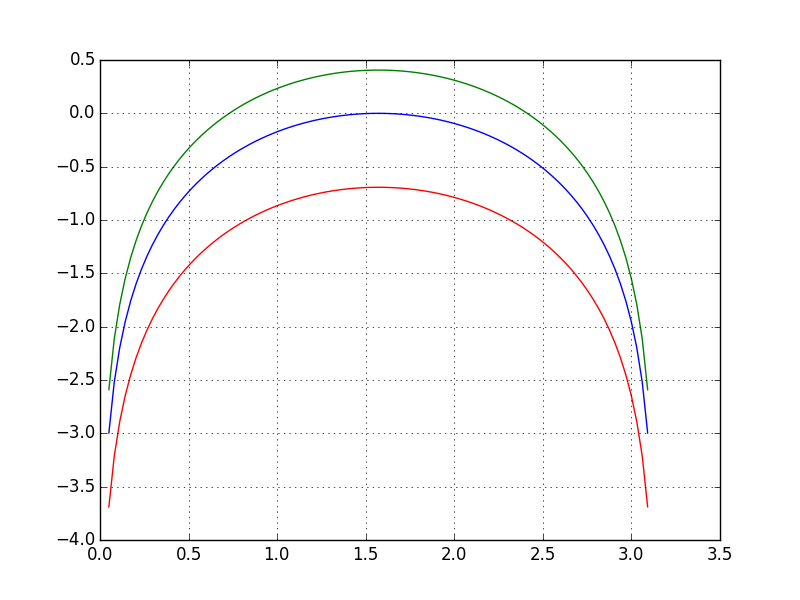
\includegraphics[scale=0.7]{images/euler_log_sine.png}
\end{figure}
